\begin{appendices}
\chapter{Few-body matrix-elements}
\label{app:ME}
This section provides the detailed $2\leftrightarrow 2$ and $2\leftrightarrow 3$ matrix-elements we used in the transport model.
The $2\leftrightarrow 2$ results are standard, and we do not re-derive them here.
A detailed derivation for the $2\leftrightarrow 3$ cross-sections is attached.

\subsection{$2\leftrightarrow 2$ processes}
The two-body scatterings between quarks, antiquarks, and gluons are standard, and we quote the results from existing references \cite{RevModPhys.59.465}.
For a light parton scattering, we keep only $\hat{t}$-channel contribution, the $\hat{s}$ and $\hat{u}$ channel contribution are suppressed at high energy.
\begin{eqnarray}
\overline{|M_{q_1q_2\rightarrow q_1q_2}|^2} &=& \frac{64\pi^2 \alpha_s^2}{9} \frac{s^2+u^2}{t^2} \\
\overline{|M_{gg\rightarrow gg}|^2} &\approx& 72\pi^2 \alpha_s^2 \frac{-su}{t^2}
 \\
\overline{|M_{qg\rightarrow qg}|^2} &\approx& 16\pi^2 \alpha_s^2 \frac{s^2+u^2}{t^2}
\end{eqnarray}
For the heavy quark, since we are interested in its diffusion dynamics at low $p_T$, we uses the exact leading order matrix-element in the vacuum.
\begin{eqnarray}
\overline{|M_{Qq\rightarrow Qq}|^2} &=& \frac{64\pi^2\alpha_s^2}{9} \frac{(M^2-u)^2 + (s-M^2)^2 + 2 M^2 t}{t^2}
\nonumber
\\
\overline{|M_{Qq\rightarrow Qq}|^2} &=& \pi^2 \left\{
32\alpha_s^2 \frac{(s-M^2)(M^2-u)}{t^2} \right.
\nonumber
\\
&+&\frac{64}{9}\alpha_s^2 \frac{(s-M^2)(M^2-u)+2M^2(s+M^2)}{(s-M^2)^2} \nonumber
\\
&+&\frac{64}{9}\alpha_s^2 \frac{(s-M^2)(M^2-u)+2M^2(u+M^2)}{(M^2-u)^2} \nonumber
\\
&+& \frac{16}{9}\alpha_s^2 \frac{M^2(4M^2 - t)}{(M^2-u)(s-M^2)} 
\nonumber
\\
&+& 16 \alpha_s^2 \frac{(s-M^2)(M^2-u)+M^2(s-u)}{t(s-M^2)}
\nonumber
\\
&-& \left. 16 \alpha_s^2 \frac{(s-M^2)(M^2-u)-M^2(s-u)}{t(M^2-u)}\right\}
\end{eqnarray}

\begin{figure}
\singlespacing
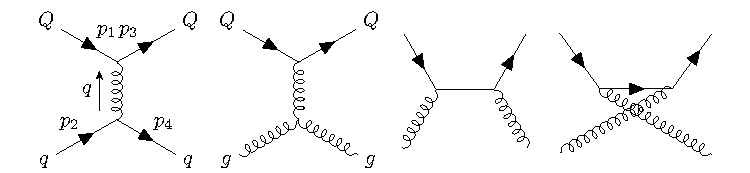
\includegraphics[width=\textwidth]{feynman.pdf}
\caption[Elastic processes: The first diagram corresponds to heavy quark]{Elastic processes: The first diagram corresponds to heavy quark ($Q$) - light quark ($q$, $\bar{q}$) scattering. The last three diagrams contribute to heavy quark ($Q$) - gluon ($g$) scattering.}\label{plots:feyn-elastic}
\end{figure}

\subsection{$2\rightarrow 3$ matrix-elements}
Large-Q $2\rightarrow 3$ inelastic processes are $g + i \rightarrow q+\bar{q} + i$, $q+i\rightarrow q+g+i$ and $g+i\rightarrow g+g+i$, where $i$ stands for a medium parton, and the other symbols stands for hard partons.
In the medium frame, the hard parton has an energy $E\gg T$, while the medium thermal parton has $E\sim T$, and the typical center-of-mass energy is $\sqrt{6ET}$.
We perform the calculation in the center-of-mass frame of the two incoming partons and let the hard parton move towards the $+z$ direction with momentum $p_1$, and the medium parton moving to the $-z$ direction with $p_2$.
The hard parton then splits into two daughter partons with momenta $k$ and $p_1 + q - k$.
The momentum transfer $q$ between the hard parton and the medium parton is thought to be large enough $|q| > Q_{\textrm{cut}}$ so we neglect the thermal correction to its propagator.

Our derivation largely follows the work of \cite{Fochler:2013epa} while relaxing the soft approximation $xq_\perp \ll k_\perp$ in \cite{Fochler:2013epa}, and we only use the collinear approximation $k_\perp^2, q_\perp^2 \ll x(1-x) \hat{s}$ with $x = k^+/\sqrt{s} = k_\perp e^y_k /\sqrt{s}$.
Also, we only include the contributions with a $\hat{t}$-channel momentum exchange between the medium and the hard partons.
The collinear approximation requires $y_k \gg \ln(k_\perp/\sqrt{s})$ so that $y_k$ cannot be arbitrarily small and $y_k>0>\gg -\ln(\sqrt{s}/k_\perp)$ is a reasonable range of application.
Because $\hat{s}\sim 6 ET$, we expect this approximation to break down when either the typical values of $q_\perp^2$ becomes comparable to $x(1-x)6ET$ or when $y_k<0$ ($x < k_\perp/\sqrt{s} \sim k_\perp/\sqrt{6ET}$).
We shall briefly mention the treatment of the $y_k<0$ region in the end.

The light-cone momentum for $p_1$ , $p_2$ and $k$ can written down directly using $\sqrt{s}$, $x$ and $k_\perp$, then applying the above collinear condition, the expression for $q$ (and therefore $p_3$ and $p_4$) is obtained by kinematic constraint up to corrections of order $\{k_\perp, q_\perp^2\}/x(1-x)\hat{s}$.
\begin{eqnarray}
p_1 &=& (\sqrt{s}, 0, \vec{0})\\
p_2 &=& (0, \sqrt{s}, \vec{0})\\
k &=& (x\sqrt{s}, \frac{k_\perp^2}{x\sqrt{s}}, \vec{k}_\perp)\\
q &\sim& (-\frac{q_\perp^2}{\sqrt{s}}, \frac{q_\perp^2 + k_\perp^2/x - 
2\vec{q}_\perp \cdot \vec{k}_\perp}{(1-x)\sqrt{s}}, \vec{k}_\perp)
\end{eqnarray}
Using the light-cone gauge with a light-like vector $n = (0, 1, 0)$, the gauge fixing condition $n\cdot A =0$ eliminates the ``+" component in the gluon (with momentum $p$) polarization vector, and is obtained by applying the transverse condition $\epsilon \cdot p = 0$ (up to a higher order correction to its normalization)
\begin{eqnarray}
\epsilon(p) &\sim& (0, \frac{2\vec{\epsilon}_\perp\cdot\vec{p}_\perp}{p^+}, \vec{\epsilon}_\perp).
\end{eqnarray}
With these preparations, the matrix-element is factorized into an amplitude for the splitting process (approximated in the collinear limit) times the amplitude for two-body collision with the medium parton.
We shall only derive explicitly the cases where the medium parton is a quark, for colliding with medium anti-quark and gluon, it is sufficient to replace the $H+q\xrightarrow{\hat{t}} H+q$ amplitude by $H+\bar{q}\xrightarrow{\hat{t}} H+\bar{q}$ and $H+g\xrightarrow{\hat{t}} H+g$.
In the end, we elucidate the connection of these results and the Bethe-Heitler limit of the solution to the AMY integral equation.

\paragraph*{Gluon splitting to quark-anti-quark pair}
\begin{figure}
\singlespacing
\centering
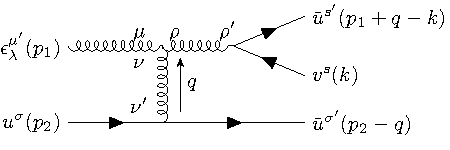
\includegraphics[width=.5\textwidth]{Large-Q-g2qqbar-A.pdf}\\
\vspace{1em}
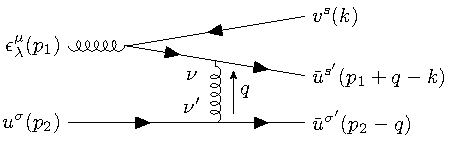
\includegraphics[width=.49\textwidth]{Large-Q-g2qqbar-B.pdf}\hfill
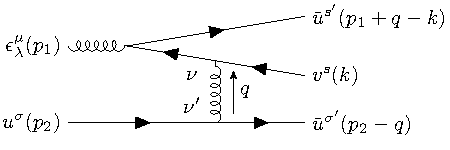
\includegraphics[width=.49\textwidth]{Large-Q-g2qqbar-C.pdf}
\caption[Three diagrams $A$ (Top), $B$ (Bottom left), $C$ (Bottom right) that]{Three diagrams $A$ (Top), $B$ (Bottom left), $C$ (Bottom right) that contribute to the large angle scattering induced gluon splitting into quark-anti-quark pair in the forward region of the center-of-mass frame.}
\label{fig:feyn-g2qqbar}
\end{figure}

Three Feynman diagrams contribute to the kinematic region $y_k >0$ in the current approximation, as shown in figure \ref{fig:feyn-g2qqbar}.
We start from the amplitude for diagram $A$.
\begin{eqnarray}
i M_A &=& (-ig)^2(-g)f^{abc}(t^b)_{j'j}(t^c)_{i'i} \epsilon_\lambda^\mu(p_1) \\\nonumber
&&\frac{-i}{(p_1+q)^2}\left(g^{\rho\rho'}-\frac{n^{\rho}(p_1+q)^{\rho'}+n^{\rho'}(p_1+q)^\rho}{n\cdot (p_1+q)}\right) \bar{u}^s(p_1+q-k)\gamma_{\rho'}v^{s'}(k) \\ \nonumber
&&\frac{-i}{q^2}\left(g^{\nu\nu'}-\frac{n^{\nu}q^{\nu'}+n^{\nu'}q^\nu}{n\cdot q}\right) \bar{u}^{\sigma}(p_4)\gamma_{\nu'}u^{\sigma'}(p_2) \\ \nonumber
&& \left[g_{\mu\nu}(p_1-q)_\rho + g_{\nu\rho}(2q+p_1)_\rho + g_{\rho\mu}(-2p_1 -q)_\nu \right]
\end{eqnarray}
Next, express the projection matrix of the gluon propagator with momentum $p_1+q$ by the sum of tensor products of its polarization vectors, and identify the amplitude $iP_{A,\lambda'}^{ss'}$ for a gluon with polarization $\lambda'$ to split into the quark and anti-quark pair with spin $s$ and $s'$.
Also, use the high energy approximation to replace $\bar{u}^i(a)\gamma^\alpha u^j(b)$ by $(a+b)^\alpha \delta^{ij}$, then
\begin{eqnarray}
i M_A &\approx& -g^3 f^{abc}(t^b)_{j'j}(t^c)_{i'i} \delta^{\sigma\sigma'} \epsilon^\mu(p_1) \\\nonumber
&&\frac{1}{(p_1+q)^2} \sum_{\lambda'=\pm}\epsilon_{\lambda'}^{\rho}(p_1+q)\underbrace{\epsilon_{\lambda'}^{*,\rho'}(p_1+q) \bar{u}^s(p_1+q-k)\gamma_{\rho'}v^{s'}(k)}_{iP_{A,\lambda'}^{ss'}} \\ \nonumber
&&\frac{1}{q_\perp^2}\left(g^{\nu\nu'}-\frac{n^{\nu}q^{\nu'}+n^{\nu'}q^\nu}{n\cdot q}\right) (2p_2-q)_{\nu'} \\ \nonumber
&& \left[g_{\mu\nu}(p_1-q)_\rho + g_{\nu\rho}(2q+p_1)_\rho + g_{\rho\mu}(-2p_1 -q)_\nu \right] \\
&=& -g^3 f^{abc}(t^b)_{j'j}(t^c)_{i'i} \frac{1}{(p_1+q)^2}\frac{1}{q_\perp^2} \sum_{\lambda'=\pm}iP_{A,\lambda}^{ss'} \delta^{\sigma\sigma'}  \\ \nonumber
&& \epsilon_\lambda^\mu(p_1)2p_2^{\nu} \epsilon_{\lambda'}^{\rho}(p_1+q) \left[g_{\mu\nu}(p_1-q)_\rho + g_{\nu\rho}(2q+p_1)_\rho + g_{\rho\mu}(-2p_1 -q)_\nu \right].
\end{eqnarray}
Finally, we evaluate the contraction in the second line using the expression for $p_1, q$ and $\epsilon$, and keep only terms that are leading in $q_\perp^2/s$ to get,
\begin{eqnarray}
i M_A \approx -g^3 f^{abc}(t^b)_{j'j}(t^c)_{i'i}\delta^{\sigma\sigma'}\frac{2s}{q_\perp^2} \frac{x(1-x)}{(\vec{k}_\perp-x \vec{q}_\perp)^2} iP_{A,\lambda}^{ss'}.
\end{eqnarray}

Diagram B and C are similar, so we only write down diagram B in detail.
\begin{eqnarray}
i M_B &=& (-ig)^3 (t^bt^a)_{i'i}(t^b)_{j'j} \epsilon_\lambda^\mu(p_1) \\\nonumber
&&\frac{-i}{q^2}\left(g^{\nu\nu'}-\frac{n^{\nu}q^{\nu'}+n^{\nu'}q^\nu}{n\cdot q}\right) \\\nonumber
&&\bar{u}^s(p_1+q-k)\gamma_{\nu}\frac{i(\slashed{p_1}-\slashed{k})}{(p_1-k)^2}\gamma^{\mu}v^{s'}(k) \\ \nonumber
&&\bar{u}^{\sigma}(p_4)\gamma_{\nu'}u^{\sigma'}(p_2)
\end{eqnarray}
Again, we represent the tensor structure of the fermion propagator by the sum of tensor products of the spinors, identify the splitting amplitude $iP_{B,\lambda'}^{ss'}$ and use the high energy limit of the current,
\begin{eqnarray}
i M_B &\approx& ig^3 (t^bt^a)_{i'i}(t^b)_{j'j}  \\\nonumber
&&\frac{-i}{q_\perp^2}\left(g^{\nu\nu'}-\frac{n^{\nu}q^{\nu'}+n^{\nu'}q^\nu}{n\cdot q}\right) (2p_2-q)_\nu' \\\nonumber
&&\frac{1}{2p_1\cdot k} \sum_\sigma \bar{u}^s(p_1+q-k)\gamma_{\nu} u^{\sigma}(p_1-k) \underbrace{\epsilon_\lambda^\mu(p_1)\bar{u}^{\sigma}(p_1-k) \gamma^{\mu}v^{s'}(k)}_{iP_{B,\lambda}^{\sigma s'}}\\
&\approx& ig^3 (t^bt^a)_{i'i}(t^b)_{j'j} \frac{-i}{q_\perp^2}\frac{1}{2p_1\cdot k} iP_{B,\lambda}^{ss'}\\\nonumber
&&\left(g^{\nu\nu'}-\frac{n^{\nu}q^{\nu'}+n^{\nu'}q^\nu}{n\cdot q}\right) (2p_2-q)_{\nu'} (2p_1-q+2k)_\nu 
\end{eqnarray}
Note that $iP_{B}$ is different from $iP_{A}$ as the initial splitting parton has a different transverse momentum from diagram $A$.
Finally, we evaluate the contraction and get,
\begin{eqnarray}
i M_B &=& i g^3 (t^b t^a)){i'i} t^b{j'j} \delta^{\sigma\sigma'} \frac{2s}{q_\perp^2} \frac{x(1-x)}{k_\perp^2}  iP_{B,\lambda}^{ss'}
\end{eqnarray}
Diagram C can be obtained similarly,
\begin{eqnarray}
i M_C &=& -i g^3 (t^a t^b)){i'i} t^b{j'j} \delta^{\sigma\sigma'} \frac{2s}{q_\perp^2} \frac{x(1-x)}{(\vec{k}_\perp-\vec{q}_\perp)^2}  iP_{C,\lambda}^{ss'} 
\end{eqnarray}
To sum the contributions from all three diagrams, apply $f^{abc}t^c = -i[t^a, t^b]$ to $iM_A$, and the result is,
\begin{eqnarray}
i (M_A+M_B+M_C) &=& ig^3 \frac{2s}{q_\perp^2} (t^b)_{j'j} x(1-x)\\\nonumber
&&\left\{(t^a t^b)_{i'i} \left(\frac{iP_{A,\lambda}^{ss'} }{(\vec{k}_\perp-x \vec{q}_\perp)^2} - \frac{iP_{C,\lambda}^{ss'}}{(\vec{k}_\perp-\vec{q}_\perp)^2}\right) \right. \\\nonumber
&&\left.-(t^a t^b)_{i'i}\left(\frac{iP_{A,\lambda}^{ss'} }{(\vec{k}_\perp-x \vec{q}_\perp)^2} - \frac{iP_{B,\lambda}^{ss'}}{k_\perp^2}\right) \right\}
\end{eqnarray}

Now we have to address what those splitting amplitudes are.
Label the four momenta as $p_g = c$, $p_q = a$, $p_{\bar{q}} = b$, then use the following representation for the spinors,
\begin{eqnarray}
u^s(p) = (\sqrt{p\cdot \sigma} \xi^s, \sqrt{p\cdot \bar{\sigma}} \xi^s)^T
v^s(p) = (\sqrt{p\cdot \sigma} \eta^s, -\sqrt{p\cdot \bar{\sigma}} \eta^s)^T.
\end{eqnarray}
$\sigma_{i=\{1,2,3\}}$ are Pauli matrices, $\sigma = (1_{2\times 2}, \vec{\sigma})$, and $\bar{\sigma} = (1_{2\times 2}, -\vec{\sigma})$.
The square root of the matrix is,
\begin{eqnarray}
\sqrt{p\cdot \sigma} =
\left.
\begin{bmatrix}
p^- & -p_L^\perp \\
-p_R^\perp & p^+
\end{bmatrix}\right.^{1/2} 
= \frac{1}{\sqrt{2(E\pm M)}}(p\cdot\sigma \pm \mathbf{1}M)\\
\sqrt{p\cdot \bar{\sigma}} =
\left.
\begin{bmatrix}
p^+ & p_\perp^- \\
p_R^\perp & p^-
\end{bmatrix}\right.^{1/2} 
= \frac{1}{\sqrt{2(E\pm M)}}(p\cdot\bar{\sigma} \pm \mathbf{1}M)\\
\end{eqnarray}
where $M$ is the mass of the particle, $p^\pm = E\pm p_z$, and $p_{R,L}^\perp = p_x \pm  i p_y$.
Currently, we only consider the massless case, and the splitting amplitude is,
\begin{eqnarray}
&&\epsilon_{\lambda, \mu}(c) \bar{u}_s(a)\gamma^\mu v_{s'}(b)\\
&=&\frac{1}{\sqrt{2a}\sqrt{2b}}(\xi^T_s a\cdot\sigma, \xi^T_{s} a\cdot \bar{\sigma})
\begin{bmatrix}
\epsilon\cdot\bar{\sigma} & 0 \\
0 & \epsilon\cdot\sigma
\end{bmatrix}
\begin{bmatrix}
b\cdot\sigma \eta_{s'}\\
b\cdot\bar{\sigma} \eta_{s'}
\end{bmatrix}
\\
&=&\frac{1}{2\sqrt{ab}}
\xi_s^T
\begin{bmatrix}
a^- & -a^\perp_L \\
-a^\perp_R & a^+
\end{bmatrix}
\begin{bmatrix}
0 & \sqrt{2}\delta_{\lambda R}\\
\sqrt{2}\delta_{\lambda L} & \frac{\sqrt{2}c^\perp_\lambda}{c^+}
\end{bmatrix}
\begin{bmatrix}
b^- & -b^\perp_L \\
-b^\perp_R & b^-
\end{bmatrix}
\eta_{s'}\\\nonumber
&-&
\frac{1}{2\sqrt{ab}}
\xi_s^T
\begin{bmatrix}
a^+ & a^\perp_L \\
a^\perp_R & a^-
\end{bmatrix}
\begin{bmatrix}
\frac{\sqrt{2}c^\perp_\lambda}{c^+} & -\sqrt{2}\delta_{\lambda R}\\
-\sqrt{2}\delta_{\lambda L} & 0
\end{bmatrix}
\begin{bmatrix}
b^+ & b^\perp_L \\
b^\perp_R & b^-
\end{bmatrix}
\eta_{s'}
\\
&=&\frac{1}{\sqrt{2ab}}
\xi_s^T
\begin{bmatrix}
-a^\perp_L b^- \delta_{\lambda L} - a^- b^\perp_L \delta_{\lambda R} + a^\perp_L b^\perp_R\frac{c^\perp_\lambda}{c^+} &
a^\perp_L b^\perp_L \delta_{\lambda L} + a^- b^+ \delta_{\lambda R} - a^\perp_L b^+\frac{c^\perp_\lambda}{c^+}
\\
a^+ b^- \delta_{\lambda L} + a^\perp_R b^\perp_R \delta_{\lambda R} - a^+ b^\perp_R\frac{c^\perp_\lambda}{c^+} &
-a^+ b^\perp_L \delta_{\lambda L} - a^\perp_R b^+ \delta_{\lambda R} + a^+ b^+\frac{c^\perp_\lambda}{c^+}
\end{bmatrix}
\eta_{s'}\\\nonumber
&-&\frac{1}{\sqrt{2ab}}
\xi_s^T
\begin{bmatrix}
-a^\perp_L b^+ \delta_{\lambda L} - a^+ b^\perp_R \delta_{\lambda R} + a^+ b^+\frac{c^\perp_\lambda}{c^+} &
-a^\perp_L b^\perp_L \delta_{\lambda L} - a^+ b^- \delta_{\lambda R} + a^+ b^\perp_L\frac{c^\perp_\lambda}{c^+}
\\
-a^- b^+ \delta_{\lambda L} - a^\perp_R b^\perp_R \delta_{\lambda R} + a^\perp_+ b^+\frac{c^\perp_\lambda}{c^+} &
-a^- b^\perp_L \delta_{\lambda L} - a^\perp_R b^- \delta_{\lambda R} + a^\perp_R b^\perp_L\frac{c^\perp_\lambda}{c^+}
\end{bmatrix}
\eta_{s'}
\end{eqnarray}
Keep the leading terms in the collinear limit which are products of $(+)(+)$ or $(+)(\perp)$ components of the momenta, and drop terms that are of order $(+)(-)$, $(\perp)(\perp)$ and $(\perp)(-)$,
\begin{eqnarray}
&&\epsilon_{\lambda, \mu} \bar{u}_s(a)\gamma^\mu v_{s'}(b)\\
&=& \frac{1}{\sqrt{2ab}}
\xi_s^T
\begin{bmatrix}
a^\perp_L b^+ \delta_{\lambda L} + a^+ b^\perp_R \delta_{\lambda R} - a^+ b^+\frac{c^\perp_\lambda}{c^+} & 0\\
0 & -a^+ b^\perp_L \delta_{\lambda L} - a^\perp_R b^+ \delta_{\lambda R} + a^+ b^+\frac{c^\perp_\lambda}{c^+}
\end{bmatrix}
\eta_{s'}
\end{eqnarray}
There are four combinations for the possible initial state polarization and final state spins:
\begin{eqnarray}
\epsilon_{\lambda, \mu} \bar{u}_s(a)\gamma^\mu v_{s'}(b) = \frac{x\vec{a} - (1-x)\vec{b}}{\sqrt{2x(1-x)}}
\begin{cases}
x, \hfill \lambda=L, s=\uparrow\\
-(1-x), \hfill \lambda=L, s=\downarrow\\
(1-x), \hfill \lambda=R, s=\uparrow\\
-x, \hfill \lambda=R, s=\downarrow\\
\end{cases}
\end{eqnarray}
Where we have used $a^+ = (1-x)c^+, b^+ = xc^+$ and $c_\perp = a_\perp+b_\perp$.
Sum over the spins and average over polarization for the squared amplitude,
\begin{eqnarray}
\frac{1}{2}\sum_\pm |P|^2 = \frac{2(x^2 + (1-x)^2)}{x(1-x)} \left((1-x)\vec{a}_\perp-x\vec{b}_\perp\right)^2.
\end{eqnarray}
This result goes back to the standard splitting function if we compute it in the frame where $a_\perp = -b_\perp$. 
However, there is no such frame that $a_\perp = -b_\perp$ satisfies simultaneously for the splitting in diagram A, B, and C.
Therefore different amplitude needs to be inserted for each diagram, and we find
\begin{eqnarray}
\label{eq:gq2qqbarq}
\frac{\sum_{\lambda, s, s', \sigma, \sigma', a, b}|M^2|_{g+q\rightarrow q+\bar{q}+q}}{2d_F 2d_A} &=& g^4 \frac{2C_F}{d_A}\frac{4s^2 x(1-x)}{q_\perp^4}  \\\nonumber
&\times& g^2\frac{(x^2+(1-x)^2)}{2} \left(C_F \vec{A}^2 + C_F \vec{B}^2 - (2C_F- C_A)\vec{A}\cdot\vec{B}\right).
\end{eqnarray}
The vectors $\vec{A}$ and $\vec{B}$ are,
\begin{eqnarray}
\vec{A} &=& \frac{\vec{k}_\perp - x\vec{q}_\perp}{(\vec{k}_\perp - x\vec{q}_\perp)^2} -  \frac{\vec{k}_\perp - \vec{q}_\perp}{(\vec{k}_\perp - \vec{q}_\perp)^2}, \\
\vec{B} &=& \frac{\vec{k}_\perp - x\vec{q}_\perp}{(\vec{k}_\perp - x\vec{q}_\perp)^2} -  \frac{\vec{k}_\perp}{\vec{k}_\perp^2}.
\end{eqnarray}
The final squared matrix-element has been factorized into the two-body scattering part (first line) and the collinear splitting part (second line) with the desired leading order QCD splitting function. 

\paragraph*{Quark splits to quark and gluon}
\begin{figure}
\singlespacing
\centering
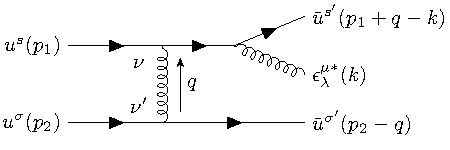
\includegraphics[width=.5\textwidth]{Large-Q-q2qg-A.pdf}\\
\vspace{1em}
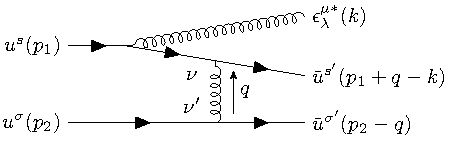
\includegraphics[width=.49\textwidth]{Large-Q-q2qg-B.pdf}\hfill
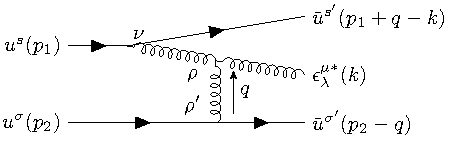
\includegraphics[width=.49\textwidth]{Large-Q-q2qg-C.pdf}
\caption[Three diagrams $A$ (Top), $B$ (Bottom left), $C$ (Bottom right) that]{Three diagrams $A$ (Top), $B$ (Bottom left), $C$ (Bottom right) that contribute to the large angle scattering induced a quark splitting into a quark and a gluon in the forward region of the center-of-mass frame.}
\label{fig:feyn-q2qg}
\end{figure}

The Feynman diagrams to be included for $q+q\rightarrow q+g+q$ are shown in Figure \ref{fig:feyn-q2qg}.
The calculation uses precisely the same technique we used for the gluon splitting channel, and we present the result directly,
\begin{eqnarray}
\label{eq:qq2qgq}
\overline{|M^2|}_{g+q\rightarrow g+g+q} &=& 
 g^4 \frac{C_F}{d_F}\frac{4s^2}{q_\perp^4}x(1-x) \\\nonumber
&\times&g^2\frac{1+(1-x)^2}{x}  
\left(C_F\vec{A}^2 + C_F\vec{B}^2 - \left(2C_F-C_A\right)\vec{A}\cdot\vec{B}\right)\\
\vec{A} &=& \frac{\vec{k}_\perp - \vec{q}_\perp}{(\vec{k}_\perp - \vec{q}_\perp)^2} -  \frac{\vec{k}_\perp - x\vec{q}_\perp}{(\vec{k}_\perp - x\vec{q}_\perp)^2} \\
\vec{B} &=& \frac{\vec{k}_\perp - \vec{q}_\perp}{(\vec{k}_\perp - \vec{q}_\perp)^2} -  \frac{\vec{k}_\perp}{\vec{k}_\perp^2}
\end{eqnarray}


\paragraph*{Gluon splitting to two gluons}
\begin{figure}
\singlespacing
\centering
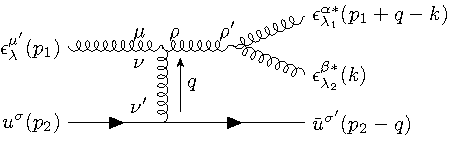
\includegraphics[width=.5\textwidth]{Large-Q-g2gg-A.pdf}\\
\vspace{1em}
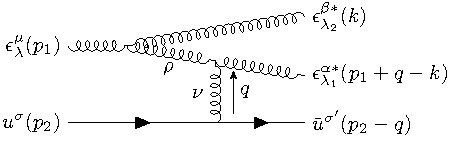
\includegraphics[width=.49\textwidth]{Large-Q-g2gg-B.pdf}\hfill
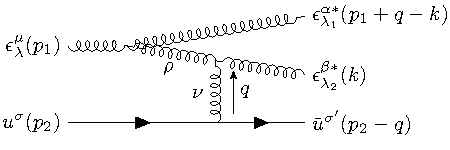
\includegraphics[width=.49\textwidth]{Large-Q-g2gg-C.pdf}
\caption[Three diagrams $A$ (Top), $B$ (Bottom left), $C$ (Bottom right) that]{Three diagrams $A$ (Top), $B$ (Bottom left), $C$ (Bottom right) that contribute to the large angle scattering induced gluon splitting into two gluons in the forward region of the center-of-mass frame.}
\label{fig:feyn-g2gg}
\end{figure}

Finally, for $g+q\rightarrow g+q+g$, the Feynman diagrams are shown in Figure \ref{fig:feyn-g2gg}. 
The simplification of the two-body collision amplitude can be done similarly as the previous two channels. 
We only write down the splitting amplitude $g\rightarrow g+ g$ in detail.
Suppressing the color index, we label the initial gluon with $\epsilon_1^\mu(p)$, and the two daughter gluons with $\epsilon_2^\nu(k)$ and $\epsilon_3^\rho(q)$.
The splitting amplitudes are then (omitting the factor $-gf^{abc}$)
\begin{eqnarray}
iP &=& \epsilon^\mu_1\epsilon^\nu_2\epsilon^\rho_3
\left[
g_{\mu\nu} (p+k)_{\rho} +  g_{\nu\rho} (p+k)_{\mu} + g_{\rho\mu} (-q-p)_{\nu}
\right]\\
&=& -\vec{\epsilon}_{1,\perp}\cdot \vec{\epsilon}_{2,\perp} \left[(p+k)^+\frac{\vec{\epsilon}_{3,\perp}\cdot \vec{q}_\perp}{q^+} - \vec{\epsilon}_{3,\perp}\cdot (\vec{p}_\perp+\vec{k}_\perp)\right] \\\nonumber
&&-\vec{\epsilon}_{2,\perp}\cdot \vec{\epsilon}_{3,\perp} \left[(-k+q)^+\frac{\vec{\epsilon}_{1,\perp}\cdot \vec{p}_\perp}{p^+} - \vec{\epsilon}_{1,\perp}\cdot (-\vec{k}_\perp+\vec{q}_\perp)\right]
\\\nonumber
&&-\vec{\epsilon}_{3,\perp}\cdot \vec{\epsilon}_{1,\perp} \left[(-q-p)^+\frac{\vec{\epsilon}_{2,\perp}\cdot \vec{k}_\perp}{k^+} - \vec{\epsilon}_{2,\perp}\cdot (-\vec{q}_\perp-\vec{p}_\perp)\right]
\end{eqnarray}
There are four possible combinations of the polarization vectors, and their respective amplitudes are,
\begin{eqnarray}
iP = \sqrt{2}\left[x\vec{q}_\perp - (1-x)\vec{k}_\perp\right]\times 
\begin{cases}
\frac{1-x+x^2}{x(1-x)}, \hfill \lambda_1=\lambda_2=\lambda_3\\
-1, \hfill \lambda_1\neq\lambda_2=\lambda_3 \\
\frac{1}{x}, \hfill \lambda_1=\lambda_3\neq\lambda_2\\
\frac{1}{1-x}, \hfill \lambda_1=\lambda_2\neq\lambda_3
\end{cases}
\end{eqnarray}
Summing over the squared amplitude of all four cases and averaging over the initial gluon polarization, one gets the desired leading order QCD splitting function,
\begin{eqnarray}
2\frac{1+x^2+(1-x)^4}{x^2(1-x)^2} \left[x\vec{q}_\perp - (1-x)\vec{k}_\perp\right]^2.
\end{eqnarray}
Substituting the amplitude in each diagram, the final squared matrix-element is 
\begin{eqnarray}
\label{eq:gq2ggq}
\overline{|M^2|}_{g+q\rightarrow g+g+q} &=&
g^4 \frac{C_A}{d_F}\frac{4s^2x(1-x)}{q_\perp^4} \\\nonumber
&\times&g^2\frac{1+x^4+(1-x)^4}{x(1-x)}   
\left(C_A\vec{A}^2 + C_A\vec{B}^2 - C_A\vec{A}\cdot\vec{B}\right)\\
\vec{A} &=& \frac{\vec{k}_\perp - x\vec{q}_\perp}{(\vec{k}_\perp - x\vec{q}_\perp)^2} -  \frac{\vec{k}_\perp - \vec{q}_\perp}{(\vec{k}_\perp - \vec{q}_\perp)^2} \\
\vec{B} &=& \frac{\vec{k}_\perp - x\vec{q}_\perp}{(\vec{k}_\perp - x\vec{q}_\perp)^2} -  \frac{\vec{k}_\perp}{\vec{k}_\perp^2}
\end{eqnarray}

\paragraph{Regulating the $2\rightarrow 3$ squared matrix-elements}
The requirement that the few-body matrix-elements only apply to processes with $q>Q_{\textrm{cut}}$ removes the divergence in the $q$ integration.
The collinear divergence when $k$ approaches $q$ or $xq$ is regulated by including a gluon thermal mass. 
In practice, the collinear divergence is further regulated by the LPM effect.
The cross-section is obtained by integrating over the final-state phase-space, parameterized by $k_\perp^2$, the rapidity of $k$ in the center-of-mass frame $y_k$, and the solid angle of the recoil medium particle.

\paragraph{Soft limit: the Gunion-Bertsch approximation}
The result we obtained for the $g\rightarrow g+g$ and $q\rightarrow q+g$ channel have a soft limit that goes back to the well known Gunion-Bertsch form. 
In the soft limit, we require the radiated gluon energy to be small enough such that $xq_\perp \ll k_\perp$.
Then, the splitting amplitudes for both $g\rightarrow g+g$ and  $q\rightarrow q+g$ are simplified into the same form,
\begin{eqnarray}
\overline{|M|}^2_{22} x(1-x)g^2 \frac{2(1-x+O(x^2))}{x} C_A \left(\frac{\vec{k}_\perp}{k_\perp^2}-\frac{\vec{k}_\perp-\vec{q}_\perp}{(\vec{k}_\perp-\vec{q}_\perp)^2}\right)^2
\end{eqnarray}
Neglecting the $O(x^2)$ terms in the splitting function, the result is the same as the improved version of the Gunion-Bertsch cross-section \cite{Fochler:2013epa} used in the full Boltzmann partonic transport model BAMPS \cite{Xu:2004mz},
\begin{eqnarray}
\overline{|M|}^2_{22} 8\pi C_A\alpha_s (1-x)^2 \left(\frac{\vec{k}_\perp}{k_\perp^2}-\frac{\vec{k}_\perp-\vec{q}_\perp}{(\vec{k}_\perp-\vec{q}_\perp)^2}\right)^2
\end{eqnarray}

\paragraph{The backward ($y_k < 0$) region}
We have mentioned at the beginning of the derivation that the condition $k_\perp^2 < x(1-x)\hat{s}$ restricts the splitting to happen only for the parton moving in the $+z$ direction in the center-of-mass frame ($y_k > 0$).
For splittings that happen in the backward region, another set of diagrams contribute, where the splitting comes from the parton that moves in the $-z$ direction in the center-of-mass frame.
Also one needs a different gauge $A^- = 0$.
The derivation is similar to the previous ones, but with the definition of $x$ and $q$ changed to $x = k^-/\sqrt{s}$, and $q = p_1-p_3$.

To combine the results that are obtained in different regions of phase space ($y_k > 0$ and $y_k < 0$), we follow \cite{Fochler:2013epa} and defines,
\begin{eqnarray}
\bar{x} &=& \frac{(k + |k_z|)}{\sqrt{s}} = \frac{k_\perp e^{|y_k|}}{\sqrt{s}}\\ 
\bar{q} &=& \Theta(y_k)(p_2-p_4) + \Theta(-y_k)(p_1-p_3)
\end{eqnarray}
which replaces the original $x$ and $q$ in our formula, and the resultant matrix-elements can be used for both forward and backward regions.



\paragraph{Relation to the Bethe-Heitler limit of the AMY formalism}
Now we show the connection between the $2\rightarrow 3$ cross-section obtained here and the Bethe-Heitler limit of the AMY equation.
In the Bethe-Heitler limit, the AMY integral equation can be solved approximately by treating $1/\tau_f$ as the leading factor. 
One obtains the splitting rate for each different channels (denoting $\vec{a}/a^2$ as $\vec{\phi}_{a}$), 
\begin{eqnarray}
R_{q\rightarrow q+g}^{BH} &\propto& g^2 P_{qg}^{q(0)}(x) \int d k^2 d q^2 \mathcal{A}(q^2) \left\{
C_A\vec{\phi}_k\cdot\left(\vec{\phi}_k-\vec{\phi}_{k-q}\right) \right.\\\nonumber
&&+\left. (2C_F-C_A) \vec{\phi}_k\cdot\left(\vec{\phi}_k-\vec{\phi}_{k+xq}\right)
+ C_A \vec{\phi}_k\cdot\left(\vec{\phi}_k - \vec{\phi}_{k+(1-x)q}\right)
\right\}
\\
R_{g\rightarrow g+g}^{BH} &\propto& g^2 P_{gg}^{g(0)}(x) \int d k^2 d q^2 \mathcal{A}(q^2) \left\{
C_A\vec{\phi}_k\cdot\left(\vec{\phi}_k-\vec{\phi}_{k-q}\right) \right.\\\nonumber
&&+\left. C_A \vec{\phi}_k\cdot\left(\vec{\phi}_k-\vec{\phi}_{k+xq}\right)
+ C_A \vec{\phi}_k\cdot\left(\vec{\phi}_k - \vec{\phi}_{k+(1-x)q}\right)
\right\}
\\
R_{g\rightarrow q+\bar{q}}^{BH} &\propto& g^2 P_{q\bar{q}}^{g(0)}(x) \int d k^2  d q^2 \mathcal{A}(q^2) \left\{
(2C_F-C_A)\vec{\phi}_k\cdot\left(\vec{\phi}_k-\vec{\phi}_{k-q}\right) \right.\\\nonumber
&&+\left. C_A \vec{\phi}_k\cdot\left(\vec{\phi}_k-\vec{\phi}_{k+xq}\right)
+ C_A \vec{\phi}_k\cdot\left(\vec{\phi}_k - \vec{\phi}_{k+(1-x)q}\right)
\right\}
\end{eqnarray}
with the collision kernel $\mathcal{A} = g^2 T m_D^2/q^2(q^2+m_D^2)$. These expressions look different from the incoherent rate computed using the cross-section derived in the previous section; however, we would like to show that they are equivalent once integration over $dk^2$ is performed.
Therefore, the incoherent rate we used in the Boltzmann equation indeed recovers the Bethe-Heitler limit of the AMY integral equation.

To show this, we start from the $2\rightarrow 3$ rate formula using the matrix-elements from equations \ref{eq:gq2qqbarq}, \ref{eq:qq2qgq} and \ref{eq:gq2ggq}. 
For the $q\rightarrow q+g$ channel, the rate in the Boltzmann equation is,
\begin{eqnarray}
R_{q\rightarrow q+g} &\propto& g^2 P_{qg}^{q(0)}(x) \int  \frac{f(p_2)dp_2^3}{2E_2(2\pi)^3} d q^2 \frac{g^4}{q^4}\\\nonumber
&&  \int d k^2\left\{
C_F\left( \vec{\phi}_{k-q}-\vec{\phi}_{k-xq} \right)^2
+ C_F\left( \vec{\phi}_{k-q}-\vec{\phi}_{k} \right)^2\right.\\\nonumber
&&\left.
- (2C_F-C_A)\left( \vec{\phi}_{k-q}-\vec{\phi}_{k-xq} \right)\cdot \left( \vec{\phi}_{k-q}-\vec{\phi}_{k} \right)
\right\}
\end{eqnarray}
Focusing on the three products (squares) of $\vec{\phi}$s under the $dk^2$ integration, we are going to expand the first term in each product and then shift the argument of the first $\vec{\phi}$ to $k$, 
\begin{eqnarray}
R_{q\rightarrow q+g} &\propto& g^2 P_{qg}^{q(0)}(x) \int  \frac{f(p_2)dp_2^3}{2E_2(2\pi)^3} d q^2 \frac{g^4}{q^4}\\\nonumber
&&  \int d k^2\left\{
C_F\vec{\phi}_{k}\left( \vec{\phi}_{k}-\vec{\phi}_{k+(1-x)q} \right)
- C_F\vec{\phi}_{k}\left( \vec{\phi}_{k-(1-x)q}-\vec{\phi}_{k} \right)\right.
\\\nonumber
&&+ C_F\vec{\phi}_{k}\left( \vec{\phi}_{k}-\vec{\phi}_{k+q} \right)
- C_F\vec{\phi}_{k}\left( \vec{\phi}_{k-q}-\vec{\phi}_{k} \right)
\\\nonumber
&&\left.
- (2C_F-C_A)\vec{\phi}_{k}\cdot \left( \vec{\phi}_{k}-\vec{\phi}_{k+q} \right)
+(2C_F-C_A)\vec{\phi}_{k} \cdot \left( \vec{\phi}_{k-(1-x)q}-\vec{\phi}_{k+xq} \right)
\right\}
\end{eqnarray}
Next, flip the sign of $q$ under the integration.
Meanwhile, insert a $-\vec{\phi}_k +\vec{\phi}_k$ in the brackets of the last term,
\begin{eqnarray}
R_{q\rightarrow q+g} &\propto& g^2 P_{qg}^{q(0)}(x) \int  \frac{f(p_2)dp_2^3}{2E_2(2\pi)^3} d q^2 \frac{g^4}{q^4}\\\nonumber
&&  \int d k^2\left\{
2C_F\vec{\phi}_{k}\left( \vec{\phi}_{k}-\vec{\phi}_{k+(1-x)q} \right)
+ 2C_F\vec{\phi}_{k}\left( \vec{\phi}_{k}-\vec{\phi}_{k+q} \right)
\right.
\\\nonumber
&&
- (2C_F-C_A)\vec{\phi}_{k}\cdot \left( \vec{\phi}_{k}-\vec{\phi}_{k+q} \right)
+(2C_F-C_A)\vec{\phi}_{k} \cdot \left( \vec{\phi}_{k+(1-x)q} -\vec{\phi}_k \right) \\\nonumber
&&\left.+(2C_F-C_A)\vec{\phi}_{k} \cdot \left(\vec{\phi}_k-\vec{\phi}_{k+xq} \right)
\right\}
\end{eqnarray}
After this manipulation, the first (second) term cancels the $C_F$ part of the fourth (third) term, 
\begin{eqnarray}
R_{q\rightarrow q+g} &\propto& g^2 P_{qg}^{q(0)}(x) \int  \frac{f(p_2)dp_2^3}{2E_2(2\pi)^3} d q^2 \frac{g^4}{q^4}\\\nonumber
&&  \int d k^2\left\{
C_A\vec{\phi}_{k}\cdot \left( \vec{\phi}_{k}-\vec{\phi}_{k+q} \right)
+C_A\vec{\phi}_{k} \cdot \left( \vec{\phi}_k - \vec{\phi}_{k+(1-x)q}\right) \right.\\\nonumber
&&\left.+(2C_F-C_A)\vec{\phi}_{k} \cdot \left(\vec{\phi}_k-\vec{\phi}_{k+xq} \right)
\right\}
\end{eqnarray}
which is the same integration as the one obtained from the Bethe-Heitler limit of the AMY equation (neglecting the screen mass in $\mathcal{A}$ when $q^2 \gg m_D^2$)
Similarly, the equivalence also exists for the $g\rightarrow g+g$ channel and the $g\rightarrow q+\bar{q}$ channel.

%\paragraph*{Mass effect in the $2\rightarrow 3$ squared matrix-elements}
%For completeness, we briefly outline the derivation of $2\rightarrow 3$ cross-section with mass effect.
%As a remark, putting the heavy flavor mass directly into the these matrix-elements is certainly legitimate if one only focus on $2\rightarrow 3$ processes.
%But once we want to approximate the effect of multiple scatterings:
%$(n \rightarrow n+1) \approx (2 \rightarrow 3)(2 \rightarrow 2)\cdots(2 \rightarrow 2)\times \textrm{corrections}$, it is not advantageous to put the mass effect into the $(2 \rightarrow 3)$ part, but better to be included into the last step of corrections, which is the approach we used.


%First, we still work under the assumption that $M \ll E$, and will only keep terms when $M$ is making direct comparison to $k_\perp, q_\perp$.
%The kinematics are now changed to,
%\begin{eqnarray}
%p_1 &=& (\sqrt{s}, 0, \vec{0})\\
%p_2 &=& (0, \sqrt{s}, \vec{0})\\
%k &=& (x\sqrt{s}, \frac{k_\perp^2}{x\sqrt{s}}, \vec{k}_\perp)\\
%q &\sim& (-\frac{q_\perp^2\sqrt{s}}{s-M^2}, \frac{x(\vec{q}_\perp-\vec{k}_\perp)^2 + (1-x)k_\perp^2 + x^2M^2}{x(1-x)\sqrt{s}}, \vec{k}_\perp)
%\end{eqnarray}
%For the splitting amplitude, off diagonal elements of $\epsilon_{\lambda, \mu}(c) \bar{u}_s(a) \gamma^\mu v_{s'} (b)$ also need to be included for helicity flipping process. 
%Moreover,
%\begin{eqnarray}
%\sqrt{p\cdot \sigma} &=& \frac{p\cdot \sigma + M}{\sqrt{2(E+M)}} \approx \frac{p\cdot \sigma + M}{\sqrt{2E}} \\
%\sqrt{p\cdot \bar{\sigma}} &=& \frac{p\cdot \bar{\sigma} + M}{\sqrt{2(E+M)}} \approx \frac{p\cdot \bar{\sigma} + M}{\sqrt{2E}}
%\end{eqnarray}
%where we have omitted the mass in the denominator since it only involves corrections of order $M/E$.
%From this one can see that the previous calculation can be used for the massive case with the substitution  $a^\pm \rightarrow a^\pm +M$ and $b^\pm \rightarrow b^\pm +M$.
%Then, the splitting amplitude becomes,
%\begin{eqnarray}
%\epsilon_{\lambda, \mu} \bar{u}_s(a)\gamma^\mu v_{s'}(b)&=& \frac{1}{\sqrt{2ab}}
%\xi_s^T A_{ss'} \eta_{s'}\\
%A_{\uparrow\uparrow} &=&
%\delta_{\lambda L} 2b_z a^\perp_L + \delta_{\lambda R} 2a_z b^\perp_R + \frac{c^\perp_\lambda}{c^+} (a^\perp_L b^\perp_R - a^+ b^+) \\
%A_{\downarrow\downarrow} &=&
%-\delta_{\lambda L}2a_z b^\perp_L - \delta_{\lambda R}2b_z a^\perp_R - \frac{c^\perp_\lambda}{c^+} (a^\perp_R b^\perp_L - a^+ b^+) \\
%A_{\uparrow\downarrow} &=&
%\delta_{\lambda L} 2a^\perp_L b^\perp_L + \delta_{\lambda R} (a^+b^-+a^-b^+) - \frac{c^\perp_\lambda}{c^+} (a^+b^\perp + a^\perp b^+) \\
%A_{\downarrow\uparrow} &=&
% \delta_{\lambda L} (a^+b^-+a^-b^+) + \delta_{\lambda L} 2a^\perp_R b^\perp_R - \frac{c^\perp_\lambda}{c^+} (a^+b^\perp + a^\perp b^+) 
%\end{eqnarray}
\end{appendices}
